\documentclass[11pt]{article}
\usepackage[margin=1in]{geometry}
\usepackage{amsmath}
\usepackage{booktabs}
\usepackage{graphicx}
\usepackage{xcolor}
\usepackage{caption}
\usepackage[
  colorlinks=true,
  linkcolor=blue!50!black,
  urlcolor=blue!50!black,
  citecolor=blue!50!black
]{hyperref}
\captionsetup{font=small}
\newcommand{\pass}{\textcolor{green!55!black}{pass}}
\newcommand{\warn}{\textcolor{orange!85!black}{warn}}
\newcommand{\fail}{\textcolor{red!75!black}{fail}}
\newcommand{\notvalidated}{\textcolor{gray}{not validated}}

\title{\textbf{Janus Resilience Lab}\\[4pt]
\large An independent reimplementation, validation, and analysis platform\\
for the Project Janus collapse--recovery model}
\author{Janus Observatory experiments track}
\date{August 21, 2026 \,\textperiodcentered\, dataset jrl-dataset-1.0.0}

\begin{document}
\maketitle

\begin{abstract}
\noindent
This report documents an experiments-track platform built around the published
collapse--recovery model of JANUS-PAPER-05 (\texttt{arXiv:2604.13774v1}, CC BY 4.0).
The model is reimplemented independently from its equations in three mutually
validating representations - exact renewal recursions, a year-by-year simulator, and an
event-driven sampler - and validated against every aggregate the source reports in
prose. On that foundation the experiment adds censoring-aware survival analysis,
variance-based global sensitivity analysis, a 65{,}536-run continuous-parameter
dataset, a surrogate benchmark under progressively harder holdout protocols, and the
paper's technosignature observation-probability equation applied to reimplemented duty
cycles. The ten Project Janus scenarios are self-consistent possibilities, not
forecasts: nothing here ranks them, assigns them probabilities, or implies they are
equally likely.
\end{abstract}

\tableofcontents

\section{The published model}
\label{sec:model}

JANUS-PAPER-05 models a technological civilization through two state variables -
technological capacity $T(t)$, initialised at $T_0 = 1$, and a resource stock $R(t)$ -
over a fixed window of 1000 years discretized into yearly steps. During active steps
technology grows linearly and resources deplete at a constant rate,
\begin{align}
  T_{t+1} &= T_t + r, &
  R_{t+1} &= R_t - \delta .
\end{align}
A collapse is triggered either by exhaustion ($R_t \le 0$) or by a per-step Bernoulli
existential hazard with rate $h$, evaluated independently of resource levels. A collapse
multiplies technology by the survival fraction $c_f$, zeroes resources, and starts a
dormant recovery period of $\mathrm{rd}$ years after which resources are restored to
$\mathrm{rf} \cdot R_0$. The \emph{duty cycle} is the fraction of active years; the
paper-style mean time to first collapse assigns the full window to runs that never
collapse.

\begin{table}[ht]
\centering
\caption{Scenario anchor parameters (canonical transcription of Table 4,
JANUS-PAPER-05).}
\small
\begin{tabular}{lccccccc}
\toprule
Scenario & $r$ & $R_0$ & $\delta$ & $c_f$ & rd (yr) & rf & $h$ \\
\midrule
S1 & 0.0020 & 400 & 1.2 & 0.6 & 40 & 0.15 & 0.003 \\
S2 & 0.0026 & 700 & 1.5 & 0.3 & 70 & 0.1 & 0.001 \\
S3 & 0.0001 & 2400 & 0 & 1 & 0 & 1 & 0 \\
S4 & 0.0060 & 600 & 2.5 & 0.2 & 100 & 0.1 & 0 \\
S5 & 0.0003 & 2500 & 0.1 & 0.9 & 20 & 0.8 & 0.0005 \\
S6 & 0.0018 & 1600 & 1 & 0.4 & 50 & 0.25 & 0.005 \\
S7 & 0.0060 & 400 & 1.5 & 0.3 & 60 & 0.2 & 0.001 \\
S8 & 0.0015 & 800 & 1.3 & 0.6 & 70 & 0.35 & 0 \\
S9 & 0.0011 & 900 & 1.3 & 0.5 & 70 & 0.35 & 0 \\
S10 & 0.0002 & 2700 & 0 & 1 & 0 & 1 & 0 \\
\bottomrule
\end{tabular}
\end{table}

Monte Carlo replication follows the published uncertainty scheme (Table 5 of the same
source): $R_0$ and $\delta$ normal with standard deviation 5\% of the mean, $c_f$ and rf
triangular over mode $\pm 5\%$ clamped to $[0,1]$, rd normal with a 10-year standard
deviation truncated at zero, and $r$ and $h$ held fixed per scenario.

\section{Replication of published outcomes}
\label{sec:replication}

Each scenario is replicated twice: a 200-run batch seeded like the paper's documented
generator seed for direct comparability, and a
20000-run ensemble whose Monte Carlo error is small
enough to expose systematic semantic
differences. Table~\ref{tab:replication-wide} compares ensemble aggregates against
every prose-reported value; Table~\ref{tab:replication-detail} lists each comparison
with its tolerance. The overall verdict is \pass.
Shaded bands in Figure~\ref{fig:replication} show the tolerances; S3 and S10 must
match exactly and do.

\begin{table}[ht]
\centering
\caption{Ours / reported, by scenario (large ensembles). ``---'' marks values the
source shows only in a figure.}
\small
\begin{tabular}{lccccl}
\toprule
Scenario & Duty cycle & First collapse (yr) & Collapse count & Never collapsed & Verdict \\
\midrule
S1 & 0.631 / --- & 211 / --- & 9.72 / 10.00 & 0.000 / 0.000 & \pass \\
S2 & 0.611 / --- & 374 / --- & 5.95 / --- & 0.000 / 0.000 & \pass \\
S3 & 1.000 / 1.000 & 1000 / 1000 & 0.00 / 0.00 & 1.000 / 1.000 & \pass \\
S4 & 0.382 / 0.381 & 241 / --- & 6.63 / 6.60 & 0.000 / 0.000 & \pass \\
S5 & 0.990 / 0.990 & 786 / --- & 0.50 / --- & 0.607 / 0.660 & \pass \\
S6 & 0.793 / --- & 199 / --- & 4.28 / 4.50 & 0.006 / 0.000 & \pass \\
S7 & 0.580 / 0.570 & 234 / 223 & 7.38 / 7.50 & 0.000 / 0.000 & \pass \\
S8 & 0.873 / 0.870 & 618 / --- & 1.94 / 2.00 & 0.000 / 0.000 & \pass \\
S9 & 0.911 / 0.910 & 694 / 689 & 1.47 / 1.50 & 0.000 / 0.000 & \pass \\
S10 & 1.000 / 1.000 & 1000 / 1000 & 0.00 / 0.00 & 1.000 / 1.000 & \pass \\
\bottomrule
\end{tabular}
\label{tab:replication-wide}
\end{table}

\begin{table}[ht]
\centering
\caption{Individual metric comparisons.}
\scriptsize
\begin{tabular}{llccccc}
\toprule
Scenario & Metric & Ours & Reported & Abs.\ diff. & Tolerance & Verdict \\
\midrule
S1 & fraction\_never\_collapsed & 0.0000 & 0.0000 & 0.0000 & 0.080 & \pass \\
S1 & mean\_collapse\_count & 9.7162 & 10.0000 & 0.2838 & 1.200 & \pass \\
S2 & fraction\_never\_collapsed & 0.0000 & 0.0000 & 0.0000 & 0.080 & \pass \\
S3 & fraction\_never\_collapsed & 1.0000 & 1.0000 & 0.0000 & 0.000 & \pass \\
S3 & mean\_duty\_cycle & 1.0000 & 1.0000 & 0.0000 & 0.000 & \pass \\
S3 & mean\_time\_to\_first\_collapse & 1000.0000 & 1000.0000 & 0.0000 & 0.000 & \pass \\
S3 & mean\_collapse\_count & 0.0000 & 0.0000 & 0.0000 & 1.200 & \pass \\
S4 & fraction\_never\_collapsed & 0.0000 & 0.0000 & 0.0000 & 0.080 & \pass \\
S4 & mean\_duty\_cycle & 0.3817 & 0.3810 & 0.0007 & 0.050 & \pass \\
S4 & mean\_collapse\_count & 6.6346 & 6.6000 & 0.0346 & 1.200 & \pass \\
S5 & fraction\_never\_collapsed & 0.6073 & 0.6600 & 0.0527 & 0.080 & \pass \\
S5 & mean\_duty\_cycle & 0.9903 & 0.9900 & 0.0003 & 0.050 & \pass \\
S6 & fraction\_never\_collapsed & 0.0063 & 0.0000 & 0.0063 & 0.080 & \pass \\
S6 & mean\_collapse\_count & 4.2767 & 4.5000 & 0.2233 & 1.125 & \pass \\
S7 & fraction\_never\_collapsed & 0.0000 & 0.0000 & 0.0000 & 0.080 & \pass \\
S7 & mean\_duty\_cycle & 0.5802 & 0.5700 & 0.0102 & 0.050 & \pass \\
S7 & mean\_time\_to\_first\_collapse & 234.2971 & 223.0000 & 11.2971 & 45.000 & \pass \\
S7 & mean\_collapse\_count & 7.3768 & 7.5000 & 0.1232 & 1.200 & \pass \\
S8 & fraction\_never\_collapsed & 0.0000 & 0.0000 & 0.0000 & 0.080 & \pass \\
S8 & mean\_duty\_cycle & 0.8726 & 0.8700 & 0.0026 & 0.050 & \pass \\
S8 & mean\_collapse\_count & 1.9446 & 2.0000 & 0.0554 & 0.500 & \pass \\
S9 & fraction\_never\_collapsed & 0.0000 & 0.0000 & 0.0000 & 0.080 & \pass \\
S9 & mean\_duty\_cycle & 0.9112 & 0.9100 & 0.0012 & 0.050 & \pass \\
S9 & mean\_time\_to\_first\_collapse & 694.4534 & 689.0000 & 5.4534 & 45.000 & \pass \\
S9 & mean\_collapse\_count & 1.4670 & 1.5000 & 0.0330 & 0.375 & \pass \\
S10 & fraction\_never\_collapsed & 1.0000 & 1.0000 & 0.0000 & 0.000 & \pass \\
S10 & mean\_duty\_cycle & 1.0000 & 1.0000 & 0.0000 & 0.000 & \pass \\
S10 & mean\_time\_to\_first\_collapse & 1000.0000 & 1000.0000 & 0.0000 & 0.000 & \pass \\
S10 & mean\_collapse\_count & 0.0000 & 0.0000 & 0.0000 & 1.200 & \pass \\
\bottomrule
\end{tabular}
\label{tab:replication-detail}
\end{table}

\begin{figure}[ht]
\centering
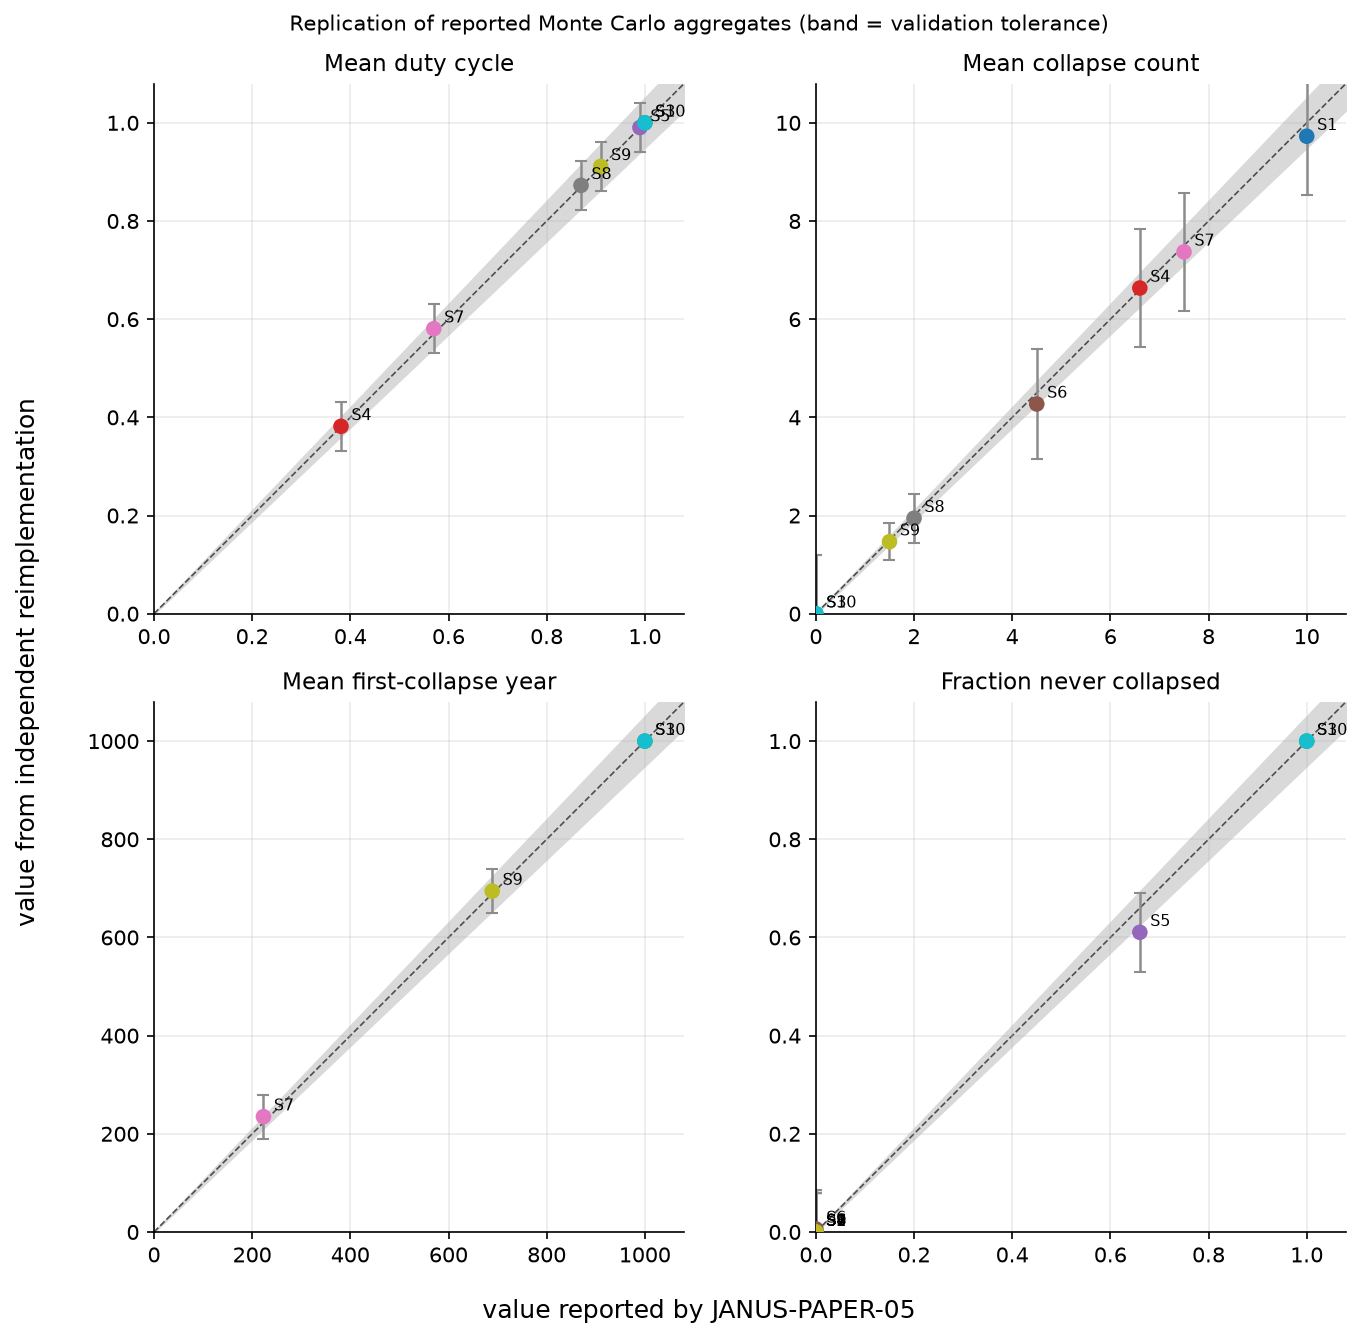
\includegraphics[width=0.82\linewidth]{../figures/fig-replication.png}
\caption{Reimplementation vs.\ reported aggregates. Error bars are validation
tolerances; the dashed line is perfect agreement.}
\label{fig:replication}
\end{figure}

\begin{figure}[ht]
\centering
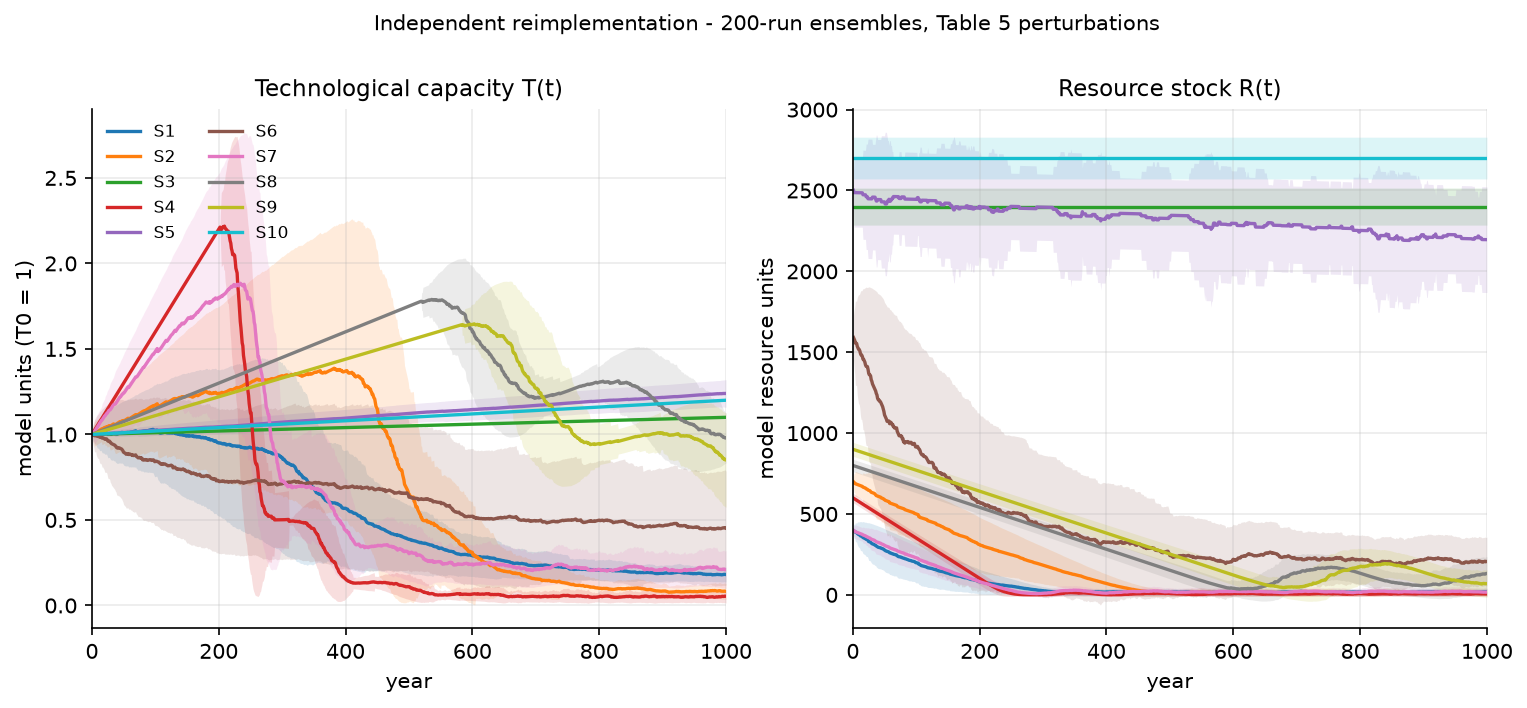
\includegraphics[width=\linewidth]{../figures/fig-trajectories.png}
\caption{Ensemble trajectories of technological capacity and resources (200 runs per
scenario, published perturbation scheme). The sawtooth pattern of S4, the late
collapses of S8/S9, and the uninterrupted growth of S3/S10 reproduce the qualitative
structure reported by the source.}
\label{fig:trajectories}
\end{figure}

One residual divergence deserves note: the never-collapsed fraction of S5 is pinned by
the model at $(1-h)^{1000} = 0.6066$, while the paper reports roughly two thirds
($\approx 0.66$) from 200 runs. Binomial noise at that ensemble size covers most of the
gap, so no semantic change was introduced to close it.

\section{Censoring-aware survival analysis}
\label{sec:survival}

The paper's truncated mean conflates ``collapsed late'' with ``never collapsed''. This
experiment therefore treats never-collapsed runs as right-censored at year 1000 and
reports Kaplan--Meier survival, Nelson--Aalen cumulative hazard, and Aalen--Johansen
cumulative incidence separating the two competing collapse causes (resource depletion
vs.\ exogenous hazard). Figure~\ref{fig:survival} shows both; the cause decomposition
recovers the expected physics - S6 is hazard-dominated, S4 collapses are almost purely
resource-driven, and S1 mixes the two.

\begin{table}[ht]
\centering
\caption{Per-scenario survival summary (20k-run ensembles). RMST = restricted mean
collapse-free time over the full window. The final two columns contrast the paper-style
truncated first-collapse mean with the censoring fraction that motivates proper
survival treatment.}
\small
\begin{tabular}{lcccccc}
\toprule
Scenario & KM median (yr) & RMST (yr) & CIF$_\mathrm{res}$(250) & CIF$_\mathrm{haz}$(250)
& Naive $T_c$ & Censored \\
\midrule
S1 & 233 & 212 & 0.000 & 0.526 & 212 & 0.000 \\
S2 & 442 & 374 & 0.000 & 0.219 & 374 & 0.000 \\
S3 & --- & 1000 & 0.000 & 0.000 & 1000 & 1.000 \\
S4 & 241 & 241 & 0.722 & 0.000 & 241 & 0.000 \\
S5 & 428 & 455 & 0.000 & 0.306 & 782 & 0.600 \\
S6 & 138 & 194 & 0.000 & 0.720 & 199 & 0.007 \\
S7 & 260 & 235 & 0.143 & 0.218 & 235 & 0.000 \\
S8 & 616 & 617 & 0.000 & 0.000 & 617 & 0.000 \\
S9 & 693 & 694 & 0.000 & 0.000 & 694 & 0.000 \\
S10 & --- & 1000 & 0.000 & 0.000 & 1000 & 1.000 \\
\bottomrule
\end{tabular}
\label{tab:survival}
\end{table}

\begin{figure}[ht]
\centering
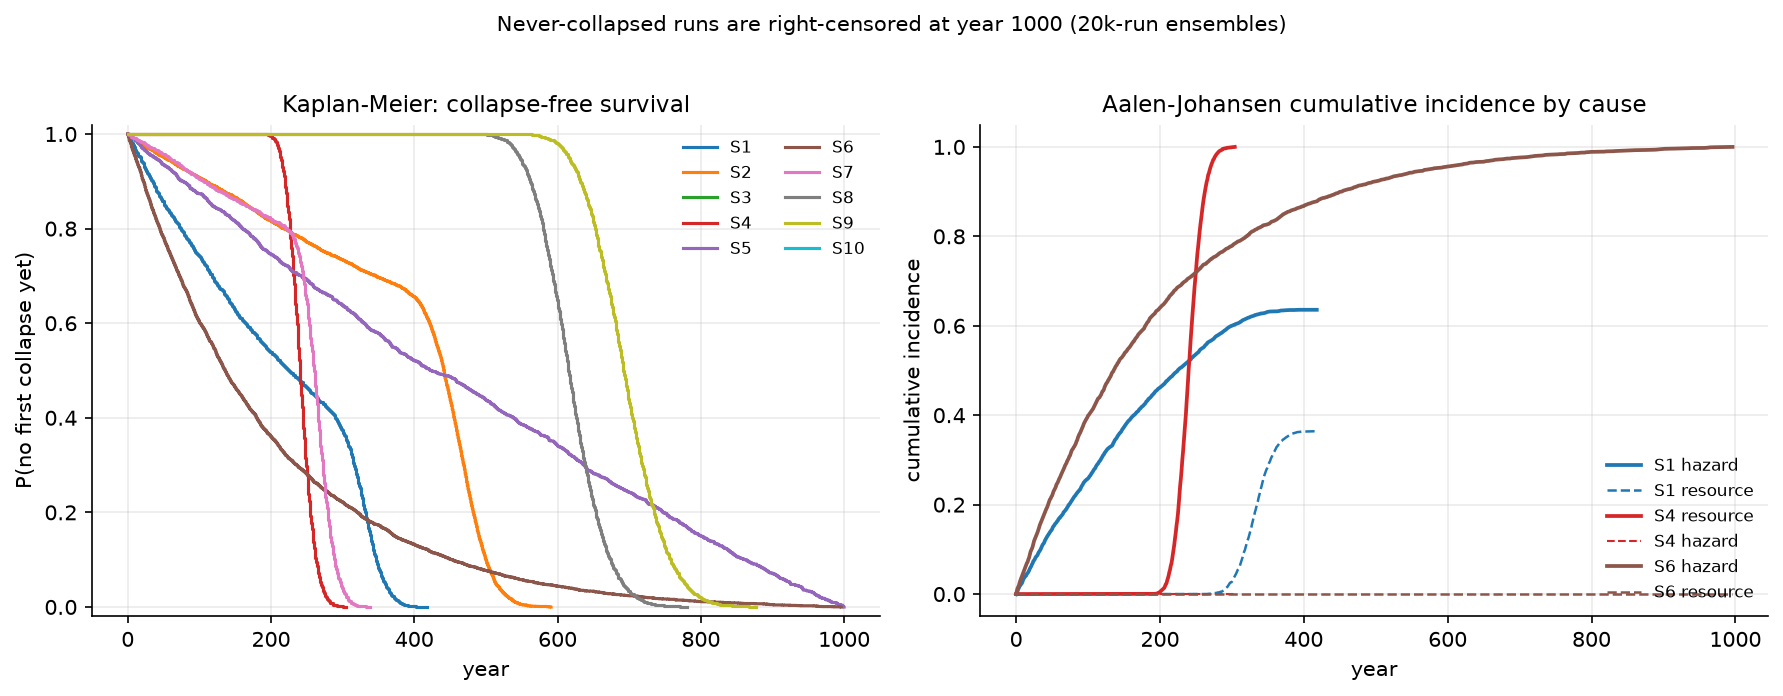
\includegraphics[width=\linewidth]{../figures/fig-survival.png}
\caption{Left: Kaplan--Meier collapse-free survival per scenario. Right:
Aalen--Johansen cumulative incidence for selected scenarios, split by cause.}
\label{fig:survival}
\end{figure}

\section{Global sensitivity analysis}
\label{sec:sensitivity}

Where the source sweeps one parameter at a time near scenario baselines, this experiment
estimates variance decomposition over the whole seven-dimensional design space using
Saltelli-style Sobol indices on independent uniform designs, replicated four times so
every estimate carries a Monte Carlo standard error, plus Morris elementary effects in
unit-cube coordinates (Figure~\ref{fig:sensitivity}).

Two structural findings act as internal consistency checks. First, the collapse fraction
$c_f$ and growth rate $r$ have exactly zero total-order effect on every timing outcome -
the model's metrics depend only on event timing, which is precisely why the paper omits
$c_f$ from its sensitivity study. Second, the exact analytic recursions and the
event-driven simulator evaluated under common random numbers produce index estimates
that agree within their standard errors (columns 1 and 2 of
Table~\ref{tab:sobol}).

By total-order effect the duty cycle is dominated by recovery delay rd and hazard $h$,
followed by $R_0$, then $\delta$ and rf; expected collapse count is dominated by $h$
(Table~\ref{tab:sobol}). Morris ranking agrees: rd, h, R0 lead, with
cf and $r$ exactly zero. These rankings answer a different question than the source's
per-scenario swings - they describe variance across the entire design space, where
interactions between parameters are active (first-order sums fall short of totals).

\begin{table}[ht]
\centering
\caption{Total-order Sobol indices (mean $\pm$ standard error over four replicates;
1024 base samples).}
\small
\begin{tabular}{lccc}
\toprule
Parameter & Analytic duty & Simulated duty (CRN) & Analytic count \\
\midrule
r & 0.000$\pm$\,0.000 & 0.000$\pm$\,0.000 & 0.000$\pm$\,0.000 \\
R0 & 0.167$\pm$\,0.011 & 0.250$\pm$\,0.012 & 0.344$\pm$\,0.035 \\
delta & 0.131$\pm$\,0.003 & 0.218$\pm$\,0.005 & 0.261$\pm$\,0.015 \\
cf & 0.000$\pm$\,0.000 & 0.000$\pm$\,0.000 & 0.000$\pm$\,0.000 \\
rd & 0.501$\pm$\,0.010 & 0.471$\pm$\,0.010 & 0.112$\pm$\,0.015 \\
rf & 0.107$\pm$\,0.011 & 0.147$\pm$\,0.010 & 0.262$\pm$\,0.015 \\
h & 0.283$\pm$\,0.019 & 0.350$\pm$\,0.017 & 0.393$\pm$\,0.017 \\
\bottomrule
\end{tabular}
\label{tab:sobol}
\end{table}

\begin{figure}[ht]
\centering
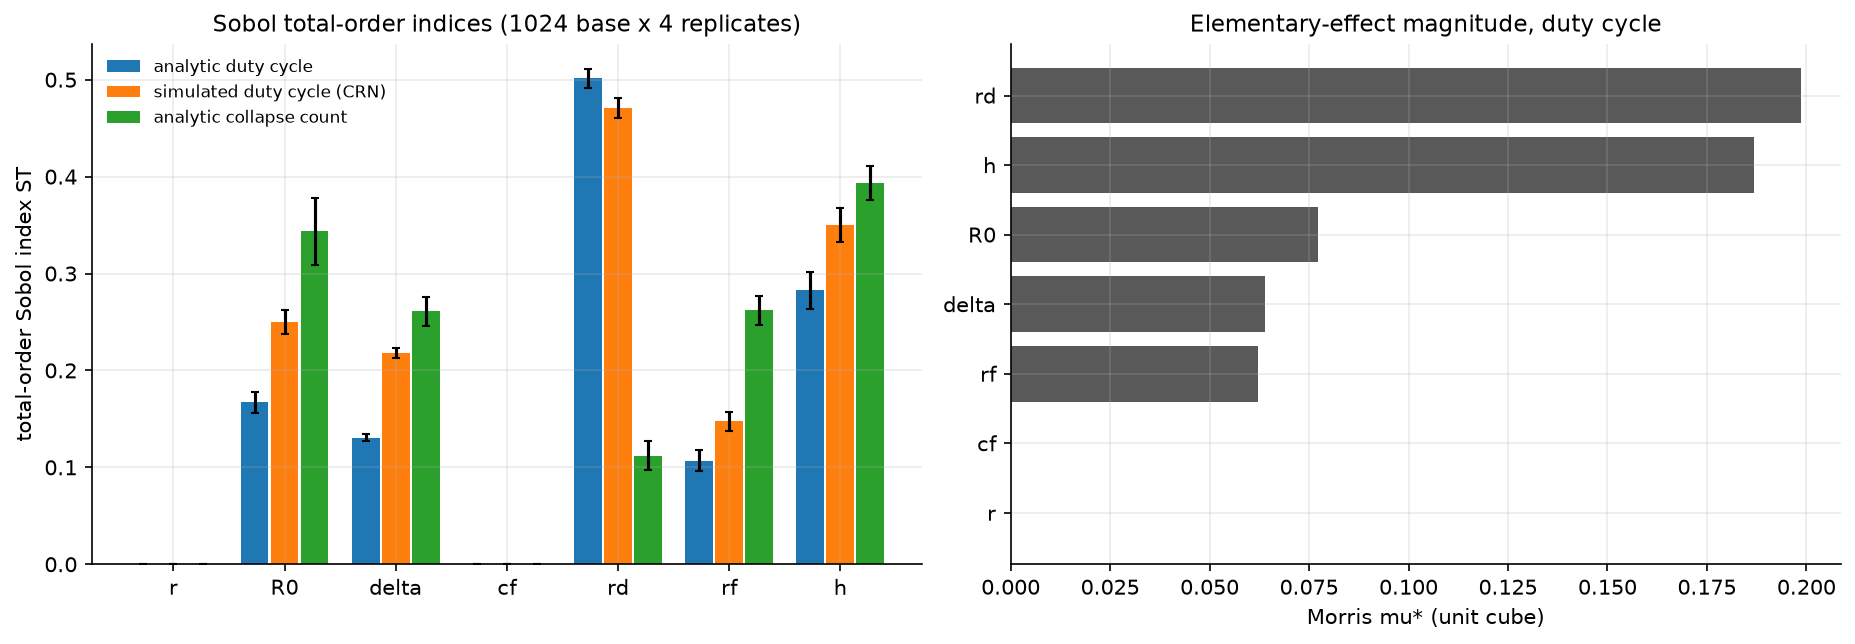
\includegraphics[width=\linewidth]{../figures/fig-sensitivity.png}
\caption{Left: total-order indices for three outputs. Right: Morris elementary-effect
magnitudes on the unit cube.}
\label{fig:sensitivity}
\end{figure}

\begin{figure}[ht]
\centering
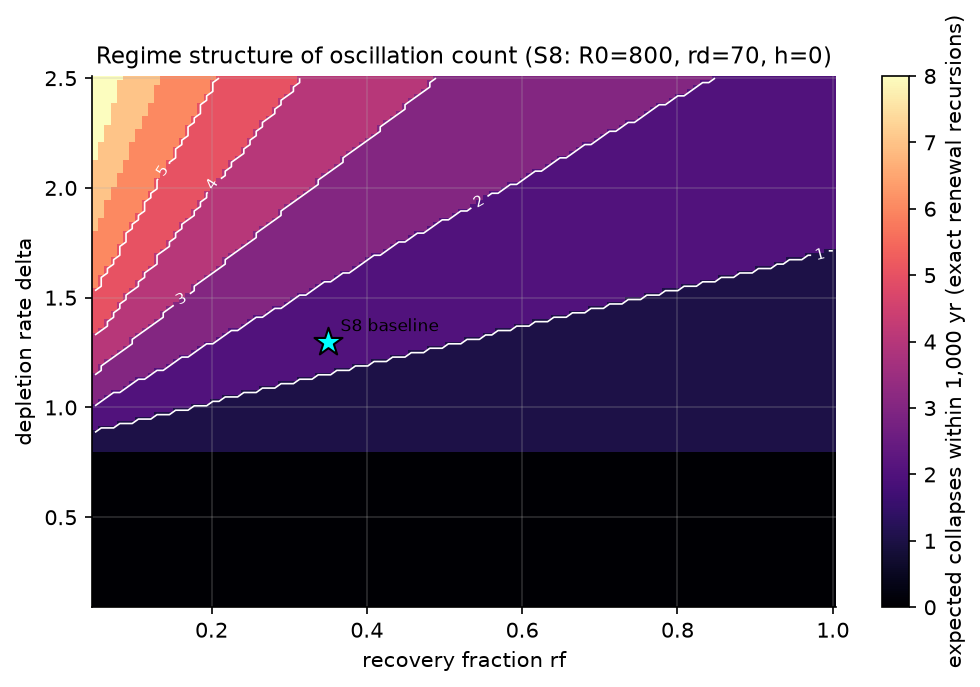
\includegraphics[width=0.9\linewidth]{../figures/fig-regime-boundary.png}
\caption{Expected number of collapse--recovery cycles across the rf--$\delta$ plane at
S8 settings, computed from the exact renewal recursions rather than Monte Carlo. The S8
baseline sits near the boundary between the two- and three-cycle regimes, matching the
source's qualitative finding.}
\label{fig:regimes}
\end{figure}

\section{Level-2 continuous-parameter dataset}
\label{sec:dataset}

The ten scenarios anchor a continuous space; they are not training examples. Version
jrl-dataset-1.0.0 contains 65,536 runs
(8,192 design points $\times$
8 seeds), sampled with a scrambled Sobol sequence over
the paper-derived bounds in Table~\ref{tab:space}, executed by the event-driven
sampler whose equivalence to the reference simulator is asserted by the test suite.
Replicate structure keeps stochastic seed noise (mean within-point sd of
0.052 duty-cycle units) separable from parameter response
(between-point spread 0.104).

\begin{table}[ht]
\centering
\caption{Design-space bounds and their provenance.}
\small
\begin{tabular}{lll}
\toprule
Parameter & Range & Source of bounds \\
\midrule
r & [0.0001, 0.006] & anchor growth rates (scenario paper Table 9) \\
R0 & [400, 2700] & anchor resource stocks \\
delta & [0.1, 2.5] & Table 6 sweep bounds \\
cf & [0.2, 1] & Table 6 joined with Table 2 governance ranges \\
rd & [0, 100] & Table 6 sweep bound; low end from Rule-by-All range \\
rf & [0.1, 1] & Table 6 low bound to full-recovery upper end \\
h & [0, 0.005] & Table 6 sweep bounds \\
\bottomrule
\end{tabular}
\label{tab:space}
\end{table}

Summary: mean duty cycle 0.868 (sd 0.120);
mean collapse count 2.93; never-collapsed fraction
0.117; among collapsed runs,
85.0\% hazard-triggered vs.\ 15.0\%
resource-depleted; regime counts 7,669 stable /
10,375 single-collapse /
47,492 recurrent
(Figure~\ref{fig:dataset-map}).

\begin{figure}[ht]
\centering
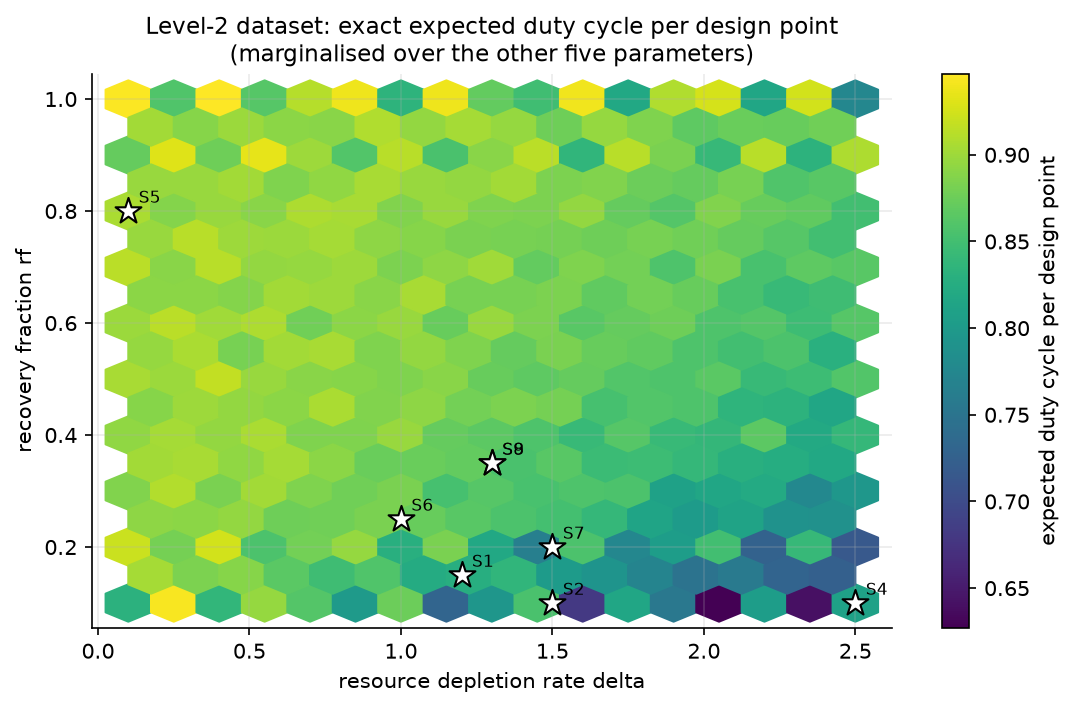
\includegraphics[width=0.95\linewidth]{../figures/fig-dataset-map.png}
\caption{Exact expected duty cycle per design point, marginalised over the other five
parameters. Scenario anchors sit inside the space except S3/S10, whose $\delta = 0$
lies on the excluded boundary.}
\label{fig:dataset-map}
\end{figure}

\section{Surrogate benchmark under grouped holdouts}
\label{sec:benchmark}

A learned model scoring well after a random split may only be rediscovering analytic
structure. Every candidate is therefore compared against the exact renewal baseline
under progressively harder protocols: a design-point-grouped random split; a contiguous
sub-box ($\delta \ge 1.8$, rf $\le 0.375$) held out entirely; and leave-one-anchor-out
folds excluding all runs within normalized radius 0.45 of each in-domain scenario
(seven folds; S3/S10 sit outside the design space). Split-conformal bands at nominal
90\% are calibrated per fold, and empirical coverage is reported next to every score.

Tables~\ref{tab:bench-duty} and~\ref{tab:bench-count} give the leaderboard as
\emph{point-level} $R^2$ (replicates averaged per design point, removing seed noise)
with conformal coverage in parentheses. Figure~\ref{fig:benchmark} visualises the
degradation pattern.

\begin{table}[ht]
\centering
\caption{Duty-cycle target: point-level $R^2$ / empirical conformal coverage, by
protocol. Negative $R^2$ means worse than predicting the test-set mean.}
\small
\begin{tabular}{lccc}
\toprule
Model & random & region block & anchor out \\
\midrule
analytic renewal & 0.954 / 0.90 & 0.975 / 0.88 & 0.932 / 0.90 \\
Gaussian process (RBF) & -0.001 / 0.87 & -0.363 / 0.66 & -7.862 / 0.81 \\
hist gradient boosting & 0.937 / 0.84 & 0.905 / 0.77 & 0.872 / 0.83 \\
ridge (quadratic) & 0.772 / 0.90 & 0.584 / 0.75 & -2.295 / 0.85 \\
\bottomrule
\end{tabular}
\label{tab:bench-duty}
\end{table}

\begin{table}[ht]
\centering
\caption{Collapse-count target: same layout.}
\small
\begin{tabular}{lccc}
\toprule
Model & random & region block & anchor out \\
\midrule
analytic renewal & 0.942 / 0.89 & 0.974 / 0.85 & 0.858 / 0.91 \\
hist gradient boosting & 0.910 / 0.83 & 0.801 / 0.73 & 0.784 / 0.86 \\
ridge (quadratic) & 0.663 / 0.90 & 0.279 / 0.72 & 0.312 / 0.89 \\
\bottomrule
\end{tabular}
\label{tab:bench-count}
\end{table}

\begin{figure}[ht]
\centering
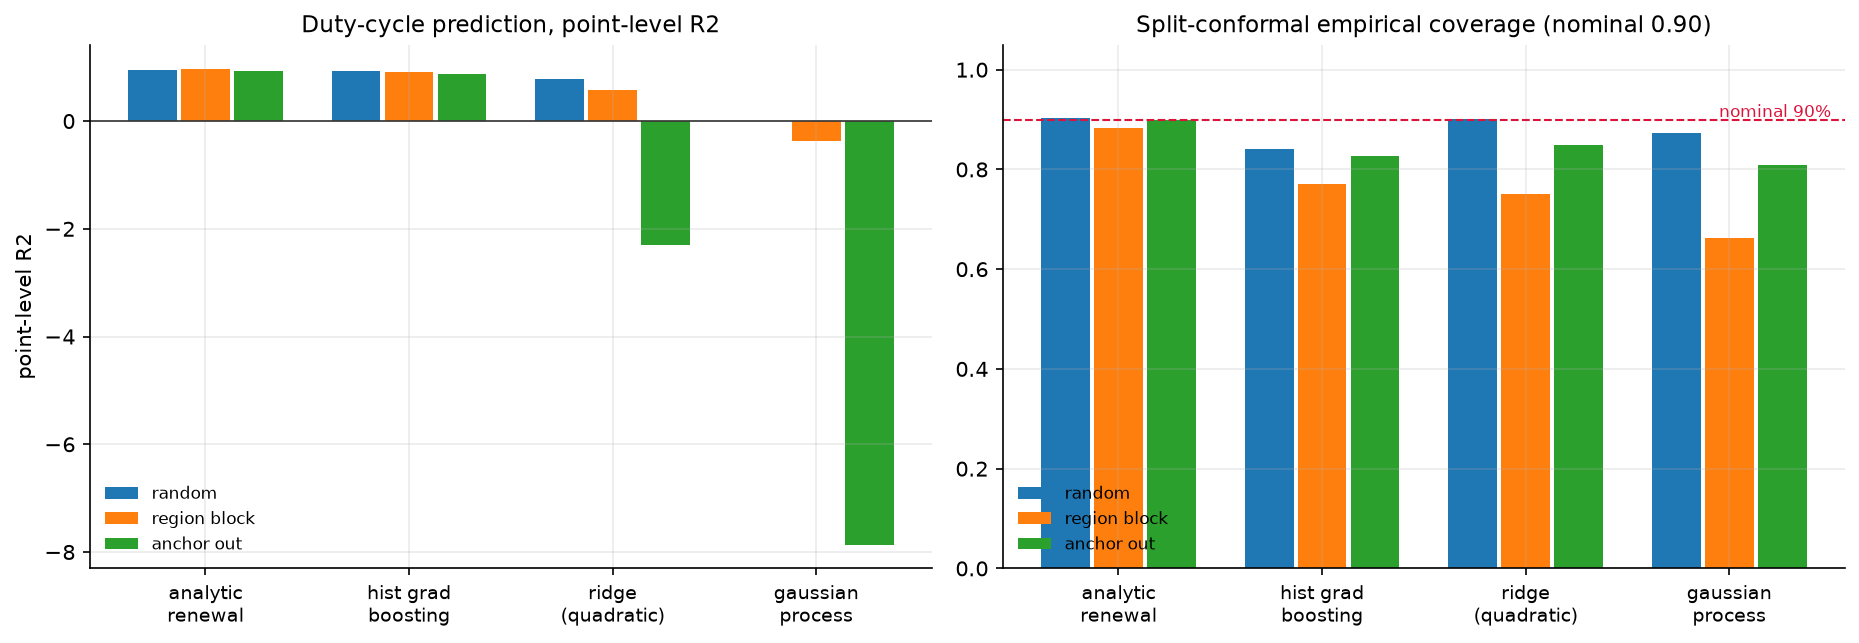
\includegraphics[width=\linewidth]{../figures/fig-surrogate.png}
\caption{Benchmark degradation (left) and conformal coverage erosion (right). The
exact analytic baseline loses almost nothing out-of-distribution because its residuals
are irreducible seed noise rather than model error.}
\label{fig:benchmark}
\end{figure}

The honest headline: the analytic baseline wins everywhere, including the easy
protocol, and learned models degrade under shift while coverage guarantees erode with
it (the Gaussian process drops to 0.66 empirical coverage in the region-block fold).
Any future claim that a learned surrogate beats this simulator must clear these
protocols first.

\section{Technosignature persistence and observation probabilities}
\label{sec:persistence}

The source defines, for technosignature $i$ present in a scenario,
\begin{equation}
  p_i \;=\;
  \left\{ D_c + \min\!\left[ T_i / T_\mathrm{span},\; 1 - D_c \right] \right\}\delta_i ,
  \qquad T_\mathrm{span} = 1000\ \mathrm{yr},
\end{equation}
so short-lived signatures track the duty cycle while long-lived relic signatures remain
observable through inactive periods. Lifetimes come from the paper's own prose (NO2
hours--days; CFC-11 55 yr; CFC-12 140 yr; CF$_4$ about 50 kyr). Presence flags are
derived here from the reviewed canonical detection matrix
(\texttt{janus.observability.apjl-figure-6}): NO2 counts present where HWO detects
CO$_2$+NO$_2$, CFCs where LIFE detects CO$_2$+CFC-11/12. CF$_4$ presence cannot be
separated from that matrix and remains explicitly \emph{not evaluated} instead of
guessed. Table~\ref{tab:persistence} and Figure~\ref{fig:persistence} use this
experiment's reimplemented duty cycles; the committed report also contains the variant
computed from canonical reported duty cycles where available.

\begin{table}[ht]
\centering
\caption{Observation probabilities $p_i$ from reimplemented duty cycles. A dash means
the presence flag is zero in the canonical detection matrix.}
\small
\begin{tabular}{lcccc}
\toprule
Scenario & $D_c$ used & NO2 & CFC-11 & CFC-12 \\
\midrule
S1 & 0.632 & 0.632 & 0.687 & 0.772 \\
S10 & 1.000 & 0.000 & 0.000 & 0.000 \\
S2 & 0.610 & 0.610 & 0.665 & 0.750 \\
S3 & 1.000 & 1.000 & 1.000 & 1.000 \\
S4 & 0.382 & 0.382 & 0.000 & 0.000 \\
S5 & 0.990 & 0.000 & 0.000 & 0.000 \\
S6 & 0.793 & 0.793 & 0.848 & 0.933 \\
S7 & 0.580 & 0.580 & 0.000 & 0.000 \\
S8 & 0.872 & 0.872 & 0.927 & 1.000 \\
S9 & 0.911 & 0.000 & 0.000 & 0.000 \\
\bottomrule
\end{tabular}
\label{tab:persistence}
\end{table}

\begin{figure}[ht]
\centering
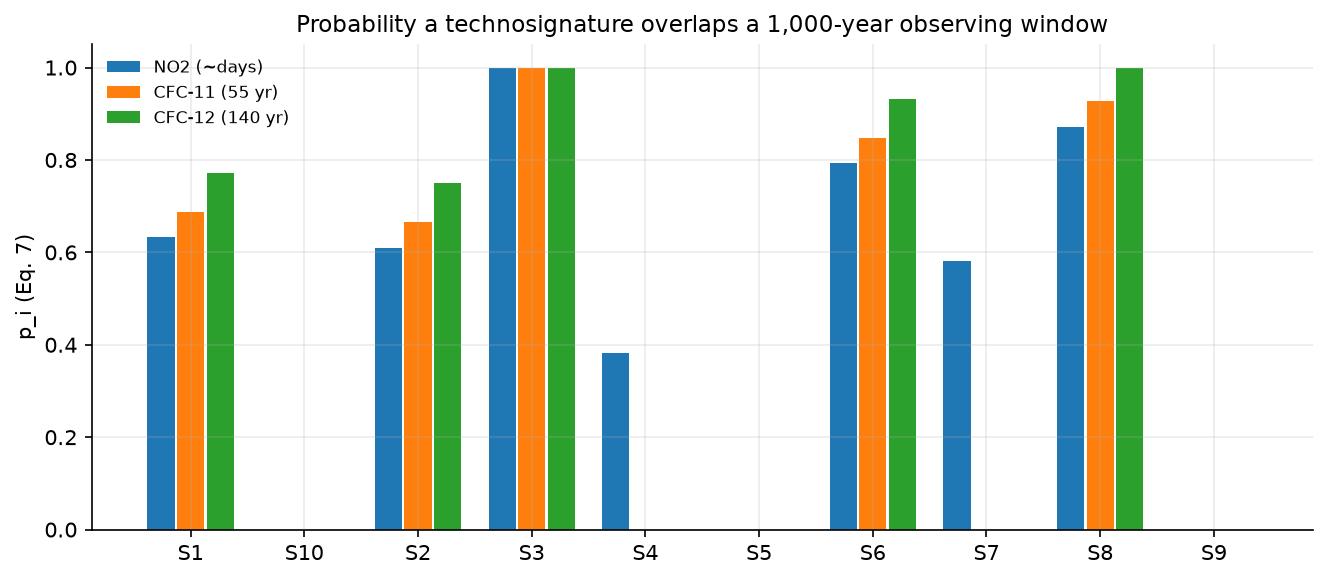
\includegraphics[width=0.98\linewidth]{../figures/fig-persistence.png}
\caption{Short-lived signatures track the duty cycle exactly; longer-lived relics add
observability during inactive periods. Scenarios lacking a canonical detection flag
show nothing regardless of duty cycle - technology does not imply detectability.}
\label{fig:persistence}
\end{figure}

\section{Adjacent NASA context data}
\label{sec:nasa}

A contextual stellar table was retrieved live from the NASA Exoplanet Archive TAP
service (24 confirmed planet-host systems within 15 pc with effective
temperatures between 5300 and 6000 K, retrieved 2026-08-21). It is
input for future observer-side work only and is not a canonical Janus dataset. Required
acknowledgment, recorded verbatim in the snapshot:

\begin{quote}
\small This research has made use of the NASA Exoplanet Archive, which is operated by the California Institute of Technology, under contract with the National Aeronautics and Space Administration under the Exoplanet Exploration Program.
\end{quote}

\section{Limitations and threats to validity}
\label{sec:limitations}

\begin{itemize}
  \item Yearly-step semantics involve ambiguities the source does not pin down
        (same-step tie-breaking, whether the collapse year counts as active). Each
        choice is recorded in \texttt{ADR-0001}, implemented identically in all three
        representations, and covered by validation tolerances.
  \item Table 5 distributions are interpreted as normal standard deviations of 5\% of
        the mean and symmetric triangular supports clamped to $[0,1]$; the source does
        not specify clamping behaviour near distribution limits.
  \item S5's never-collapsed fraction reproduces to 0.61 vs the reported $\approx
        0.66$; the analytic value is pinned at $(1-h)^{1000} = 0.6066$ and the residual
        is consistent with 200-run Monte Carlo noise.
  \item First-order Sobol indices carry wide standard errors because the product
        estimator is heavy-tailed; total-order indices are the stable ranking and are
        always printed with standard errors.
  \item Leave-one-anchor-out folds exclude S3/S10 because $\delta = 0$ sits outside
        the continuous design space, whose lower bound follows the source's own Table 6
        sweep floor.
  \item The Gaussian process baseline is deliberately frugal (single optimizer
        restart, subsampled training); its scores bound naive GP usage rather than
        best-possible GP performance.
\end{itemize}

\section{Provenance and rights}
\label{sec:provenance}

\begin{itemize}
  \item Model equations, parameters, uncertainty scheme, sweep bounds, and the
        persistence equation: JANUS-PAPER-05 (\texttt{arXiv:2604.13774v1}, CC BY
        4.0), loaded at runtime from the reviewed canonical transcription
        \texttt{data/canonical/collapse/model-and-reported-results.json}.
  \item Presence flags derived from \texttt{janus.observability.apjl-figure-6}
        (JANUS-PAPER-03, CC BY 4.0).
  \item The author-hosted \texttt{technocycles} repository is public but carries no
        license; it is cited, not copied. This reimplementation was written from the
        paper's equations alone.
  \item NASA Exoplanet Archive data carries the acknowledgment quoted in
        Section~\ref{sec:nasa}.
  \item No scenario probability, ranking, or forecast is produced anywhere in this
        pipeline.
\end{itemize}

\subsection*{Environment}

Python 3.13.5, NumPy 2.5.2, SciPy 1.18.0,
scikit-learn 1.9.0, captured 2026-08-22T00:03:24+00:00.
Git commit \texttt{unavailable}.

\appendix
\section{Reproducing every number and figure}

All artifacts regenerate deterministically from the repository state recorded in the
report headers:

\begin{tabbing}
  \texttt{uv sync --project experiments/resilience-lab --extra dev --extra ml} \\
  \texttt{uv run --project experiments/resilience-lab pytest experiments/resilience-lab/tests} \\
  \texttt{uv run --project experiments/resilience-lab janus-resilience replicate} \\
  \texttt{uv run --project experiments/resilience-lab janus-resilience survival} \\
  \texttt{uv run --project experiments/resilience-lab janus-resilience sensitivity} \\
  \texttt{uv run --project experiments/resilience-lab janus-resilience dataset} \\
  \texttt{uv run --project experiments/resilience-lab janus-resilience surrogate} \\
  \texttt{uv run --project experiments/resilience-lab janus-resilience persistence} \\
  \texttt{uv run --project experiments/resilience-lab janus-resilience figures} \\
  \texttt{uv run --project experiments/resilience-lab janus-resilience report} \\
\end{tabbing}

Every figure is re-rendered from committed JSON reports and seeded ensembles; every
table in this document was generated directly from those JSON files, not transcribed.

\end{document}
